\begin{minipage}{0.6\textwidth}

Аппроксимация распределения:
\begin{equation*}
    \sub{f}{fit}(x, y) = B+A \exp\left(
        - \left(\frac{\tilde{x}}{\sigma_1}\right)^2 - \left(\frac{\tilde{y}}{\sigma_2}\right)^2
    \right)
\end{equation*}


\end{minipage}
\hfill
\begin{minipage}{0.31\textwidth}

Полное число атомов:
\begin{equation*}
\boxed{
	N = \pi A \sigma_1 \sigma_2
}
\end{equation*}

\end{minipage}


\begin{figure}[h]
    \centering
    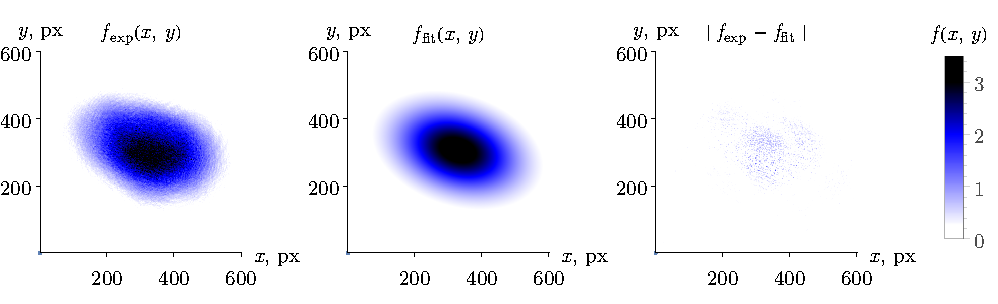
\includegraphics[width=0.8\textwidth]{../MOT/figs/fit_mot_v2.pdf}
    \caption{Экспериментально сфотографированное распределение атомов $\sub{f}{exp}$, аппроксимация распределения атомов гауссовой функцией $\sub{f}{fit}$ и остатки аппроксимации $|\sub{f}{exp} - \sub{f}{fit}|$}
    %\label{fig:}
\end{figure}
